\documentclass[letterpaper,twocolumn,10pt]{article}
\usepackage{usenix2019_v3}

% to be able to draw some self-contained figs
\usepackage{tikz}
\usepackage{amsmath}

% inlined bib file
\usepackage{filecontents}

%-------------------------------------------------------------------------------
\begin{filecontents}{\jobname.bib}
%-------------------------------------------------------------------------------
@Book{sandvineinternet,
  title =        {The Global Internet Phenomena Report},
  publisher =    {Sandvine},
  year =         2019,
  note =         {\url{https://www.sandvine.com/global-internet-phenomena-report-2019}}
}
@Book{arpachiDusseau18:osbook,
  author =       {Arpaci-Dusseau, Remzi H. and Arpaci-Dusseau Andrea C.},
  title =        {Operating Systems: Three Easy Pieces},
  publisher =    {Arpaci-Dusseau Books, LLC},
  year =         2015,
  edition =      {1.00},
  note =         {\url{http://pages.cs.wisc.edu/~remzi/OSTEP/}}
}
@InProceedings{waldspurger02,
  author =       {Waldspurger, Testing Carl A.},
  title =        {Memory resource management in {VMware ESX} server},
  booktitle =    {USENIX Symposium on Operating System Design and
                  Implementation (OSDI)},
  year =         2002,
  pages =        {181--194},
  note =         {\url{https://www.usenix.org/legacy/event/osdi02/tech/waldspurger/waldspurger.pdf}}
}
@InProceedings{ghemawatgobioffleung03:gfspaper,
  author =       {Ghemawat S., Gobioff H. and Leung S.-T.},
  title =        {The Google File System},
  booktitle =    {ACM Symposium on Operating Systems Principles},
  year =         2003,
  note =         {\url{https://static.googleusercontent.com/media/research.google.com/en//archive/gfs-sosp2003.pdf}}
}
\end{filecontents}

\hypersetup{draft}

%----------------------------------------------------------------------------sssofof  
\begin{document}
%-------------------------------------------------------------------------------

%don't want date printed
\date{}

% make title bold and 14 pt font (Latex default is non-bold, 16 pt)
\title{\Large \bf Chunky: a distributed GFS-based file store}

%for single author (just remove % characters)
\author{
{\rm Matthew Lee}\\
Stanford University
% copy the following lines to add more authors
% \and
% {\rm Name}\\
%Name Institution
} % end author

\maketitle

%-------------------------------------------------------------------------------
\begin{abstract}
%-------------------------------------------------------------------------------
  We present Chunky, a distributed file store based on the design of the Google File System (GFS)~\cite{ghemawatgobioffleung03:gfspaper}. Like GFS, Chunky replicates file chunks across multiple chunkservers for fault-tolerance and employs a single central master to coordinate access to files. Unlike GFS, Chunky implements write-once semantics for files, which simplifies the design considerably (obviating the need for a lease mechanism) while still enabling a practical, interesting system that demonstrates robustness in the face of multiple chunkserver failures.
\end{abstract}


%-------------------------------------------------------------------------------
\section{Introduction}
%-------------------------------------------------------------------------------

Designers of distributed file systems sometimes find it convenient to deviate from the traditional POSIX file API. Chunky is no exception. Motivated by the need to store more data than can fit on a single machine across multiple servers in a way that is resilient to the failure of some servers, Chunky exposes a simple file API and implements a GFS-like chunk replication scheme.

% Now we're going take a look at Section~\ref{sec:figs}, but not before

%-------------------------------------------------------------------------------
\section{Chunky: Design and API}
\label{sec:figs}
%-------------------------------------------------------------------------------

\subsection{Write-Once: Not entirely useless}

Write-once file semantics may seem too restrictive for a useful system, but on the contrary, there are in fact important classes of workloads that are essentially write-once in nature, such as content publishing. Video content alone, which by itself constitutes more than 60 percent of Internet traffic~\cite{sandvineinternet}, is a case where video files are uploaded once - written to a distributed sytem of video content hosts - and thereafter only read by clients.

More generally, write-once semantics are not actually an impediment to useful computation: the entire paradigm of functional programming manages to make do with immutable "variables".

\subsection{Chunky API}

Chunky exposes a simple API for file manipulation.

\begin{description}
  
\item[open] a function which returns a \texttt{ChunkyFile} that is a handle to data stored at \texttt{path}. At this point no space has been allocated for the data.

\item[reserve] a function that declares the size of a ChunkyFile in \texttt{bytes}, callable once per file.

\item[write] a function which writes \texttt{data} to a ChunkyFile segment given by \texttt{range}, callable once per file.

\item[read] a function which reads a \texttt{range} of data from a ChunkyFile and populates the \texttt{data} field provided by the caller.

\end{description}

\subsection{Important system interactions}

\begin{description}
  \item[Heartbeats] The chunkservers periodically send heartbeats to the master, enabling the master to detect when new chunkservers come online and when chunkservers fail. As in GFS, chunkservers are the source of truth for the chunk handles that they store; the master requests chunkservers that have just come online to send their list of chunk handles.
  \item[Chunk Handle Lookup] The master maintains a mapping from (file name, intra-file chunk index) tuples to chunk handles. This mapping is populated at the time of file allocation. The client library never caches this information; every read by a client is begun by a query to the master for the chunk handle that stores the data of a file.
  \item[Chunk Server Lookup] The master also maintains the mapping from chunk handle to a list of chunkservers that stores that chunk. This mapping is populated when chunkservers report their chunk handle lists. The client library queries the master for the chunk servers that own a particular chunk in order to read or write to the correct chunkservers.
  \item[Chunk Allocation] When the client library reserves space for a file, the master computes the number of chunks needed and chooses $k$ random chunkservers per chunk. The allocation of chunk data occurs on the chunkserver side by creating a file on the underlying Linux filesystem to store the chunk data.
  \item[Data Movement] After clients have queried the master for the list of chunkservers that own a particular chunk, data movement between the client and chunkservers occurs without the mediation of the master. Like in GFS, this design ensures that the master is never on the datapath; the master only sends control messages, which helps prevent the master from bottlenecking the entire system.
\end{description}

\subsection{Implementation trivia}

The system is implemented in C++, using gRPC for communication between components. Chunkservers store file data on the underlying filesystem in order to take advantage of sparse file support (which avoids consuming physical space for allocated but unwritten chunks). File metadata on chunkservers is stored on a LevelDB database.

\section{Evaluation}

We instantiated a system with 5 chunkservers and a replication factor of 3. To observe the effect of a chunkserver failure on the system, we triggered a crash on chunkserver 3 at about the halfway point. Later, we revived chunkserver 3.

\begin{figure*}[]
	\centering
		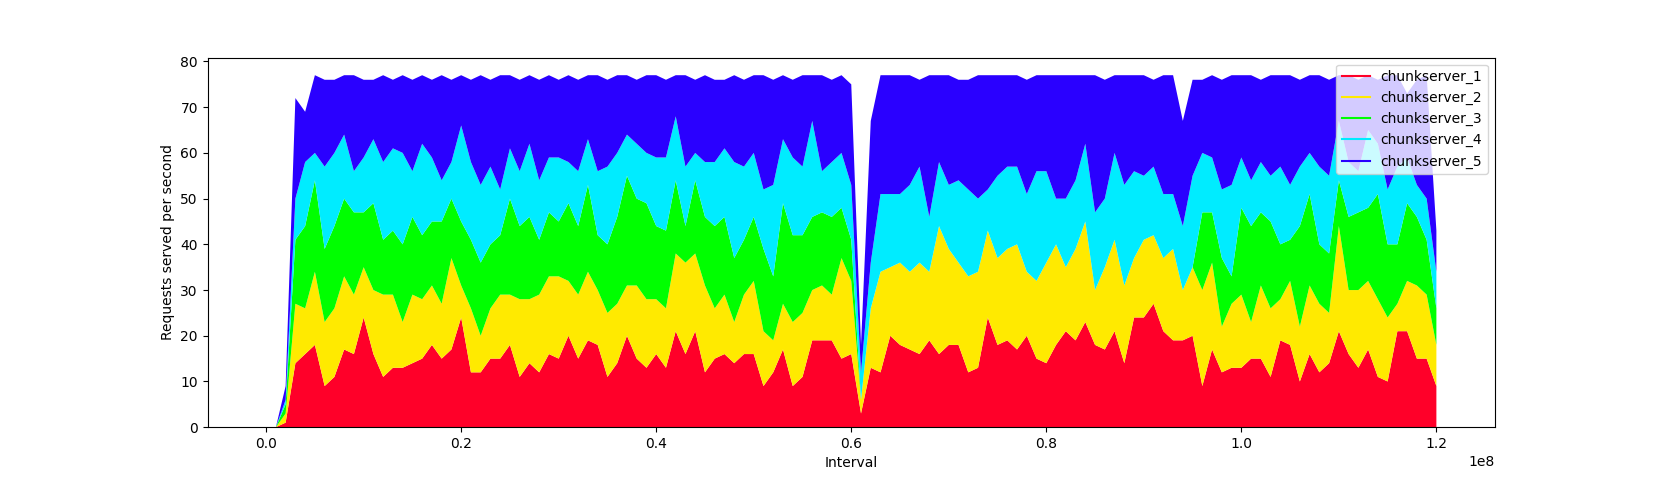
\includegraphics[width=\textwidth]{node_failure_and_recovery.png}
	\caption{Request throughput in presence of node failure and recovery} 
\end{figure*}

The figure on the following page shows the total throughput of the system in requests served per second. The failure of the chunkserver causes the total throughput to dip momentarily as the client is blocked while waiting for a request to the failed chunkserver to time out. After the master detects the failure of the chunkserver, the master deletes the failed chunkserver from its chunk handle to chunkserver mapping and therefore the client no longer attempts to send read requests to the failed chunkserver. As a result the blocking behaviour is not seen after the failure. The request load is redistributed to the other chunkservers and the total system throughput resumes. Later, when the failed chunkserver comes back online, the system returns to its former state, with all chunkservers sharing the load.

%-------------------------------------------------------------------------------
\section*{Availability}
%-------------------------------------------------------------------------------

The source and driver scripts are available at \url{https://github.com/mattlkf/chunky}.

%-------------------------------------------------------------------------------
\bibliographystyle{plain}
\bibliography{\jobname}

%%%%%%%%%%%%%%%%%%%%%%%%%%%%%%%%%%%%%%%%%%%%%%%%%%%%%%%%%%%%%%%%%%%%%%%%%%%%%%%%
\end{document}
%%%%%%%%%%%%%%%%%%%%%%%%%%%%%%%%%%%%%%%%%%%%%%%%%%%%%%%%%%%%%%%%%%%%%%%%%%%%%%%%

%%  LocalWords:  endnotes includegraphics fread ptr nobj noindent
%%  LocalWords:  pdflatex acks
